\documentclass[12pt]{article}
\usepackage{listings}
\usepackage{graphicx}
\usepackage{float}
\usepackage[margin=2cm]{geometry}
\usepackage{titlesec}
\usepackage{titling}
\usepackage{lipsum}
\usepackage{fancyhdr}
\usepackage{rotating}
\usepackage{hyperref}
\usepackage{enumitem}
\usepackage{tikz}
\usepackage{pdfpages}
\usepackage{xcolor}


\definecolor{codegreen}{rgb}{0,0.6,0}
\definecolor{codegray}{rgb}{0.5,0.5,0.5}
\definecolor{codepurple}{rgb}{0.58,0,0.82}
\definecolor{backcolour}{rgb}{0.95,0.95,0.92}

\lstdefinestyle{mystyle}{
    backgroundcolor=\color{backcolour},   
    commentstyle=\color{codegreen},
    keywordstyle=\color{magenta},
    numberstyle=\tiny\color{codegray},
    stringstyle=\color{codepurple},
    basicstyle=\ttfamily\footnotesize,
    breakatwhitespace=false,         
    breaklines=true,                 
    captionpos=b,                    
    keepspaces=true,                 
    numbers=left,                    
    numbersep=5pt,                  
    showspaces=false,                
    showstringspaces=false,
    showtabs=false,                  
    tabsize=2
}
\lstset{style=mystyle}

\graphicspath{{./resources/}}

\newcommand{\bb}[1]{\textbf{\textit{#1}}}
\newcommand{\tco}{Touriscov}

\hypersetup{
    colorlinks=true,
    linkcolor=blue,
    filecolor=magenta,      
    urlcolor=cyan,
    pdftitle={miniMBAProject},
    pdfpagemode=FullScreen,
    }

\lhead{TOURISCOV}
\chead{}
\rhead{
\includegraphics[scale=0.1]{/miniMBA.png}}
\lfoot{}
\cfoot{\thepage}
\rfoot{}

\renewcommand{\thefigure}{}

\renewcommand{\maketitle}{
\begin{center}
    \Huge\textbf{Algorithms Report} \\ 
    \vspace{1em}
    \Large\bfseries Amr Wahdan \\
    {20201615334} \\
    \Large\bfseries Bassem Akram \\
    {20201612642} \\

    \vspace{1em}
    \large December 28\textsuperscript{th}, 2024
\end{center}
}


\title{Algorithms Report}
\author{Amr Wahdan}
\date{Saturday, May 28th 2024}

\begin{document}
\pagenumbering{0}

\begin{center}
   \topskip8cm
    
\includegraphics[width=0.8\textwidth]{uniLogo.jpg}  
\end{center}
\vspace{1em}
\begin{center}
    \scalebox{2}{\Huge\textbf{Bellman--Ford}}
	\vspace{3em}
    \scalebox{2}{\Huge\textbf{Algorithm}}
\end{center}
\vspace{1em}
\maketitle
\pagenumbering{roman}
\newpage

\pagenumbering{arabic}

\section{Overview}

Graph algorithms form the foundation of computer science, enabling solutions to complex problems related to networks, routing, optimization, and data organization. Among these algorithms, the Bellman-Ford algorithm stands out as a versatile and robust method for solving the single-source shortest path problem in a weighted graph. Named after Richard Bellman and Lester Ford, who independently developed the algorithm, it has become a cornerstone in graph theory and applications. \par

\subsection{Historical Background}

The development of the Bellman-Ford algorithm dates back to the mid-20th century, a period marked by rapid advances in mathematical optimization and computer science. Its origin is attributed to the work of Richard Bellman and Lester R. Ford Jr., two prominent figures in mathematics and operations research. \par

\subsubsection{Richard Bellman}

Richard Bellman (1920–1984) was an American mathematician and a pioneer in the field of dynamic programming. He earned his Ph.D. from Princeton University in 1946 and made significant contributions to applied mathematics, operations research, and computer science. Bellman is best known for formulating the principle of optimality, which underpins dynamic programming techniques. \par

His work focused on solving complex optimization problems by breaking them into smaller subproblems, a concept that plays a crucial role in the Bellman-Ford algorithm. Bellman's approach was driven by the need to address real-world problems in economics, control systems, and logistics, where decisions often depend on sequential steps. \par

\begin{figure}[H]
	\begin{center}
		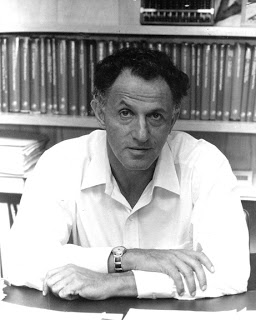
\includegraphics[width=0.3\textwidth]{Richard_Ernest_Bellman.jpeg}
	\end{center}
	\caption{Richard Ernest Bellman}\label{fig:bellman}
\end{figure}

\subsubsection{Lester R Ford}

Lester Randolph Ford Jr. (1886–1967) was an American mathematician renowned for his contributions to number theory and optimization. Ford's work laid the groundwork for algorithms that handle weighted graphs and optimization problems. Though he is often credited alongside Bellman for the algorithm, his contributions primarily focused on shortest path calculations and flow problems in network graphs.

Ford's research provided mathematical rigor and theoretical foundations for graph algorithms, enabling their application in practical scenarios involving resource distribution and routing. \par

\begin{figure}[H]
	\begin{center}
		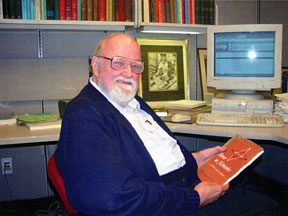
\includegraphics[width=0.6\textwidth]{lesterford.jpg}
	\end{center}
	\caption{Richard Ernest Bellman}\label{fig:ford}
\end{figure}

\subsection{Motivation for development}
The Bellman-Ford algorithm was developed to address two key challenges in graph optimization:
\begin{itemize}
	\item \textbf{Handling Negative Weights:} Traditional shortest path algorithms, like Dijkstra's algorithm, fail when graphs contain negative weights. Such weights arise in various domains, including finance (e.g., losses or rebates) and transportation (e.g., fuel savings or discounts).
	\item \textbf{Negative Cycle Detection:} Many real-world scenarios require identifying cycles with negative weights to prevent instability or exploit arbitrage opportunities. Existing algorithms at the time could not detect such cycles efficiently.
\end{itemize}

These two main issues were the main problems with Dijkstra's algorithm that Bellman \& Ford were trying to improve on.

Bellman and Ford sought a systematic approach to solve these problems, leading to the creation of an algorithm that guarantees correctness even in complex cases involving negative weights and cycles. \par


\subsection{Dijkstra's algorithm and Its Relation to the Bellman-Ford Algorithm}

Dijkstra's algorithm and the Bellman-Ford algorithm are two of the most widely studied techniques in graph theory for solving the single-source shortest path problem. Both algorithms aim to determine the shortest path from a specified starting vertex to all other vertices in a graph, yet they differ significantly in their approach, efficiency, and application. While Dijkstra's algorithm is prized for its speed and simplicity, it is constrained by its inability to handle graphs with negative edge weights. Conversely, the Bellman-Ford algorithm, though slower, is more versatile as it accommodates graphs with negative edge weights and can detect negative weight cycles. This document explores these two algorithms in detail, examining their methodologies, strengths, weaknesses, and the contexts in which each is most useful. \par

\subsubsection{Dijkstra's Algorithm: A Greedy Approach to Shortest Paths}

Dijkstra's algorithm, named after Dutch computer scientist Edsger Dijkstra, is a classic example of a greedy algorithm designed to find the shortest paths in a graph with non-negative edge weights. The algorithm leverages the principle of selecting the locally optimal choice at each step, which leads to the globally optimal solution for the shortest path problem. \par

The procedure begins by initializing the distance of the source vertex to zero and setting the distances to all other vertices as infinity. This reflects the fact that initially, no paths to these vertices have been discovered. A priority queue, often implemented using a min-heap, is used to repeatedly extract the vertex with the smallest known distance. For each vertex extracted, the algorithm examines its neighbors, updating their distances if a shorter path through the current vertex is found. This process, known as relaxation, ensures that the shortest paths are incrementally refined until all vertices have been processed. \par

The efficiency of Dijkstra's algorithm stems from its reliance on the priority queue. Using a binary heap or Fibonacci heap reduces the complexity of distance updates and extractions, making the algorithm highly scalable for dense graphs. Specifically, its time complexity is O((V + E) log V), where V represents the number of vertices and E represents the number of edges. \par

Despite its efficiency, Dijkstra's algorithm has a notable limitation—it cannot handle graphs with negative edge weights. The algorithm's greedy nature assumes that once a vertex's shortest distance is finalized, it cannot be improved. However, in graphs with negative edge weights, subsequent relaxations may invalidate this assumption, leading to incorrect results. Consequently, Dijkstra's algorithm is primarily suited for graphs with non-negative weights, such as transportation networks or routing systems. \par

\subsubsection{Bellman-Ford Algorithm: A Dynamic Approach with Greater Flexibility}

In contrast to Dijkstra's greedy approach, the Bellman-Ford algorithm employs a dynamic programming paradigm to solve the shortest path problem. Developed by Richard Bellman and Lester Ford, this algorithm is more versatile as it can handle graphs with negative edge weights and detect negative weight cycles. Its approach is iterative and systematically considers every edge, relaxing distances repeatedly until the shortest paths are guaranteed. \par

The algorithm begins similarly to Dijkstra's, initializing distances with infinity and setting the source vertex's distance to zero. It then performs a series of iterations, relaxing each edge during each pass. The process of relaxation checks whether traversing an edge yields a shorter path to its destination vertex. This relaxation is repeated V - 1 times, where V is the number of vertices in the graph. The rationale behind this repetition is rooted in the observation that the shortest path in any graph can have at most V - 1 edges. \par

A critical feature of the Bellman-Ford algorithm is its ability to detect negative weight cycles. After completing V - 1 iterations, an additional iteration is performed to check for further relaxations. If any distance can still be reduced, the graph must contain a negative weight cycle, which implies that no finite shortest path exists. This capability makes the Bellman-Ford algorithm invaluable for applications involving currency arbitrage or network routing, where negative weights may arise naturally. \par

However, this flexibility comes at a cost. The Bellman-Ford algorithm has a time complexity of O(V × E), making it slower than Dijkstra's algorithm, particularly for dense graphs. Nevertheless, its ability to handle negative weights and cycles often outweighs its performance drawbacks in scenarios where correctness is more important than speed. \par


\section{Problem Definition}

The Bellman-Ford algorithm is used to determine the shortest path from a single source vertex to all other vertices in a weighted graph. Unlike Dijkstra's algorithm, which also addresses this problem, the Bellman-Ford algorithm can handle graphs with negative weight edges. This capability makes it particularly useful for applications involving financial transactions, network routing, and flow optimization where negative weights might indicate losses, rebates, or constraints. \par

The algorithm also detects negative weight cycles—cycles in which the total sum of weights is negative. Such cycles imply that a path could continue indefinitely, reducing the total path cost, rendering the shortest path undefined. Identifying these cycles is crucial in network and financial systems where instability or arbitrage opportunities may arise. \par


\subsection{Key Features}
\begin{enumerate}
	\item Single-source shortest paths: Computes distances from one source vertex to all others. 
	\item Negative weight handling: Supports graphs with negative edge weights, unlike Dijkstra's algorithm. 
	\item Negative cycle detection: Identifies cycles with cumulative negative weights, a feature critical for certain applications. 
	\item Polynomial time complexity: Executes in O(V × E), where V represents the number of vertices and E represents the number of edges.
\end{enumerate}

\section{Algorithm Overview}
The Bellman-Ford algorithm iteratively relaxes edges to ensure that all shortest paths are computed. Relaxation is the process of updating the shortest known distance to a vertex based on its neighboring vertices. The steps are:

\begin{enumerate}
	\item \textbf{Initialization:} Set the distance to the source vertex as 0 and to all other vertices as infinity. 
	\item \textbf{Relaxation:} For each edge, update the shortest distance if a shorter path is found through that edge. Repeat this process V - 1 times (where V is the number of vertices). 
	\item \textbf{Negative Cycle Check:} Perform one additional iteration to verify if any further relaxation is possible, which would indicate the presence of a negative weight cycle.
\end{enumerate}

By systematically examining edges and improving path estimates, the Bellman-Ford algorithm guarantees correctness, even in cases where other algorithms might fail. \par 

\section{Python Code}

\lstinputlisting[language=Python, breaklines=true]{bellman_ford3.py}

\subsection{Algorithm Chart}
Note that the below chart uses estimates for the biggest input sizes since the time is in days.
\begin{figure}[H]
	\begin{center}
		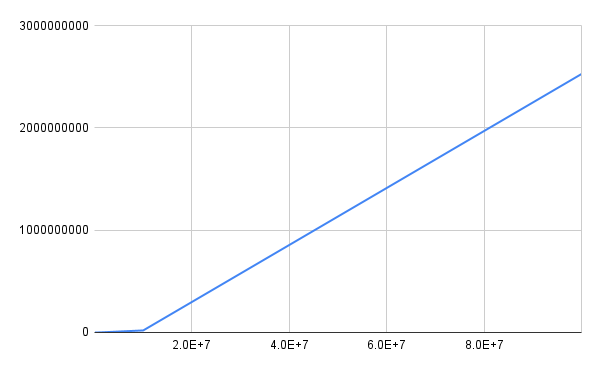
\includegraphics[width=0.95\textwidth]{chart.png}
	\end{center}
	\caption{Line chart showing time complexity of Bellman--Ford Algorithm for various inputs}\label{fig:chart}
\end{figure}

\subsection{Complexity Analysis}
To calculate the time complexity, let's break it down to its key operations:

\subsubsection{Initialization}
Setting the distance to the source vertex as 0 and all other vertices as infinity takes O(V) time.

\subsubsection{Relaxation}
\begin{enumerate}
	\item The algorithm iterates through all edges V - 1 times, as a shortest path in a graph cannot contain more than V - 1 edges.
	\item Each iteration involves E edge relaxations (checking and possibly updating the distance for each edge).
	\item Time Complexity for Relaxation:
	\[
		O((V - 1)\cdot E)=O(V\cdot E)
	\]
\end{enumerate}

\subsubsection{Negative Cycle Detection}
An additional pass through all E edges is performed to check for negative weight cycles. \par 

Time Complexity for negative cycle check is \( O(E) \)

\subsubsection{Total Time Complexity}
By summing all three steps up we get,
\[ O(VE) \]

Because it is the most dominate term of all three terms, it is the total time complexity

\subsection{Pros \& Cons}
\subsubsection{Pros}
\begin{itemize}
	\item Handles graphs with negative weights.
	\item Detects negative weight cycles, which is essential for stability checks in applications. 
	\item Simple and intuitive, making it easier to implement and adapt for different scenarios. 
\end{itemize}

\subsubsection{Cons}
\begin{itemize}
	\item Less efficient than Dijkstra's algorithm for graphs with non-negative weights, due to its O(V × E) complexity. 
	\item Not suitable for dense graphs with a large number of edges.
\end{itemize}

\section{Conclusion}
The Bellman-Ford algorithm provides a reliable and flexible approach to solving shortest path problems, particularly in scenarios involving negative weights or the need for cycle detection. Its simplicity, coupled with its ability to handle edge cases, makes it an indispensable tool in graph theory and practical applications. While it may not always be the fastest solution, its robustness ensures accuracy and applicability in fields ranging from networking and finance to logistics and optimization systems. \par

\end{document}
